%%=====================================================================================
%%
%%       Filename:  labnote.tex
%%
%%    Description:  Note about this .
%%
%%        Version:  1.0
%%        Created:  Tuesday 16 May 2017
%%       Revision:  none
%%
%%         Author:  Dilawar Singh (), dilawars@ncbs.res.in
%%   Organization:  NCBS Bangalore
%%      Copyright:  Copyright (c) 2017, Dilawar Singh
%%
%%          Notes:  
%%                
%%=====================================================================================

\RequirePackage{luatex85,shellesc}
\documentclass[a4paper]{article}
\usepackage{pgf,tikz}
\usepackage{pgfplotstable}
\usepackage{bashful}
\usepackage{amsmath}
\usepackage{amssymb}
\usepackage[sfdefault,light]{FiraSans}
\usepackage{siunitx}
\usepackage{xifthen}
\usepackage{grffile}
\usepackage{verbdef}
\usepackage{pgfplots}
\usetikzlibrary{shapes,backgrounds,decorations,decorations.markings}
\usetikzlibrary{shapes,positioning,calc,arrows,arrows.meta}
\usetikzlibrary{external}
%\tikzexternalize[prefix=./_tikz/]

\usepackage[]{glossaries}
\makeglossaries 

\title{Subunit exchange \emph{synchronises} cluster of CaMKII bistables}
\author{Dilawar Singh}
\date{\today}


\begin{document}
\maketitle

\begin{abstract}

    In this experiment, we enable diffusion on subunit x and y; and check its
    impact on switch behaviour. We find that system of N switches tend to
    synchronize with each other. Thereby making the cluster of bi-stables to behave like a  one bistable
    switch. 

    \footnote{
        This is in contract to our previous study with simple Markov chain
        based bi-stables which predicted that system of N switches likely to act as
        one \emph{almost always ON} monostable switch.
    }

    See figure \ref{fig:intermediate_state_distribution} in section \ref{sec:result}.

\end{abstract}

\newglossaryentry{intermediate_states}{
    name = {intermediate states},
    description={ For system of $N$ switches, the intermediate states are
        collection of all states where at least one switch is either \texttt{ON}
        or \texttt{OFF}. For example, for a system of 3 switches, the
        intermediate states is the set $\left( 001, 010, 100, 011, 110, 101
        \right)$ where $0$ and $1$ represents \texttt{OFF} and \texttt{ON} of
        switch respectively.
    }
}
    

\section{Experiment}
\label{sec:Experiment}

\edef\length{150e-9} \edef\radius{30e-9}
\newcommand\vol{\directlua{tex.print(3.1416 * \radius * \radius * \length);}}

We construct a 'good' bistable switch with 6 CaMKII rings and 27 PP1 (see file {\tt
./CMakeLists.txt} ) in a cylinder of length \SI{\length}{ \meter} and radius of
\SI{\radius}{\meter}  (volume = \SI{\vol}{\meter ^3}). This configuration shows
a good bistable behaviour.

We assemble N (=3) switches together and setup diffusion of subunit among them.
The subunits $x$ and $y$ diffuse between compartments as shown below.

\tikzsetnextfilename{voxels}
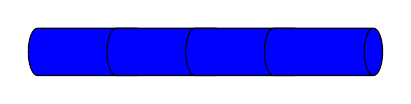
\begin{tikzpicture}[scale=1 , every node/.style={} ]
    %\draw[thick,blue,postaction={decorate}
            %,decoration={markings,mark=between positions 0 and 1 step 2cm with {
                %\node[double arrow,fill=blue!50,transform shape,minimum
                %height=10mm,minimum width=1mm,inner sep=0pt] {}; }
            %}] (0,0) circle(1.5cm and 1.5cm);

    \foreach \i in {0,1,...,3}
    {
        \node[cylinder,fill=blue,draw,minimum width=6mm, minimum height=15mm]
            (cyl_\i) at (6\i cm,0) {};
    }

\end{tikzpicture}    

We run the simulation for different values of diffusion coefficients. 

\newcommand\filn[1]{./CaMKII-6+PP1-27+L-125e-9+N-3+diff-#1.dat_processed.dat}
\foreach \diffConst in {0,1e-18,1e-15,1e-14,1e-13,1e-12}
{
    \edef\everyN{100}
    \edef\fileName{\filn{\diffConst}}
    \begin{figure}[]
        \begin{tikzpicture}[scale=1]
            \begin{axis}[ xlabel=Time(days),ylabel=Active CaMKII
                    , grid style={draw=gray!20}, grid = both
                    , width=0.5\textwidth, height = 3cm, scale only axis
                    , xmin=0
                ]
                \addplot [color=blue] gnuplot [ raw gnuplot ] {
                        plot "\fileName" using (column("time")/86400.0):"CaMKII*" 
                            every \everyN with lines;
                    };
            \end{axis}
        \end{tikzpicture}
        \begin{tikzpicture}[scale=1]
            \begin{axis}[ 
                    xlabel=Active CaMKII %, ylabel = Freq
                    , grid style={draw=gray!20}, grid = both
                    , width=3cm, height = 3cm, scale only axis
                    , ymax = 0.3
                ]
                \addplot [hist={density,bins=19},fill=blue, bar width=1pt] gnuplot[raw gnuplot] {
                        plot "\fileName" using "CaMKII*" every \everyN;
                };
        \end{axis}
    \end{tikzpicture} 
    \caption{ Diffusionn coefficient \SI{\diffConst}{\micro \meter^2 \per \second}. }
    \end{figure}
}

\section{Result}
\label{sec:result}

\subsection{Mean and variation of CaMKII activity vs diffusion coefficient}

The most important result from this experiment is the following.

\textbf{ When subunit exchange is enabled in a system of $N$ CaMKII bistables,
all bistables in the system 'synchronizes' their switching making the system a
single bistable switch. }

Figure \ref{fig:intermediate_state_distribution} shows that
\gls{intermediate_states} of $N$ switches becoming increasing scarce upon 
increasing the coupling among switches.

\begin{figure}[ht!]
    \begin{center}
        \begin{tikzpicture}[scale=1]
            \begin{semilogxaxis}[ xlabel=Diffusion Coefficient (\si{\meter^2 \per \second})
                , ylabel=\Gls{intermediate_states}
                , grid style={draw=gray!20}, grid=both ]
                \addplot+ [error bars/.cd,y dir=both,y explicit] table
                    [ col sep=comma, x=diff const
                    , y=intermediate states mean
                    , y error=intermediate states std
                    ] {./decay_of_intermediate_states.png.dat};
            \end{semilogxaxis}
        \end{tikzpicture}
    \end{center}
    \caption{Intermediate states become scarcer as we increase the 'coupling'
        among switches. Large diffusion coefficient increases the coupling among
        switches by making subunit exchange faster.
    }
    \label{fig:intermediate_state_distribution}
\end{figure}

\glsaddall
\printglossaries

\end{document}          
